\section{The Necron Tombworlds}


\subsection{Building a Necron Army}

In games of the Horus Heresy: Age of Darkness, the models under a given player’s control are referred to as that player’s army. Each army is composed of a single Force Organisation chart (most commonly using the Crusade Force Organisation chart), which will include one or more Detachments. An army whose Primary Detachment is selected from any Army List is considered to have the Faction of that Primary Detachment (for example, an army whose Primary Detachment was selected from the Necrons List would be considered an Necron army). Units from various Sub-factions cannot be mixed in the same Detachment, unless a Special Rule or other ability permits this.

Other, non-Primary, Detachments in the same army may be selected from any other Army List - following any additional restrictions applied, such as the ones on the next page - but each Detachment may only include units from a single Army List, unless another Special Rule states otherwise.

When selecting a Primary Detachment, you must also choose a Sub-Faction for that detachment, in the form of a Necron Dynasty. Each Dynasty provides special bonuses and options for their units and determines the Alliance Levels between other Sub-Factions.

In addition, each Dynasty has a number of allied units that are usually attached to its Tomb Worlds, whether that be Triarch Praetorians watching over the slumbering necrons, a Destroyer Cult filling part of their ranks, or Flayed Ones lurking at the fringes. As such, a Primary Detachment is also allowed to incorporate a number of Allied Units without requiring an entire Allied Detachment be taken, so long as the number of points spent on Triarch, Destroyer, and Flayed models does not exceed 25\% of the army's total points.

\newpage
\begin{multicols}{2}
\subsection{Force Organisation Charts and Detachments}

The maximum and minimum number of units that may be included in a given army is defined by a Force Organisation chart, of which there is one basic chart available, the Crusade Force Organisation chart. 

Any Force Organisation chart is made up of one or more Detachments. A Force Organisation chart will always include one Primary Detachment, which must be selected, and may also include a number of optional Detachments which a player may choose to use or ignore. Each Detachment that a player chooses to use as part of their army must use a single Army List, which determines the Faction of that Detachment. Most optional Detachments are not required to be the same Faction as the Primary Detachment, but some Detachments may have special rules which require them to be of a certain Faction (and thus use a specific Army List). Detachments of different Factions in the same army will have additional special rules that determine how they interact (see \hyperref[allies]{the Allied Section}).

Each Detachment is composed of a number of boxes, each linked to one of the Battlefield Roles. Each of these boxes allows the player to make one selection from the section of their Army List that includes units of the same Battlefield Role. Dark boxes indicate Compulsory selections, which must be included as part of the Detachment, while the lighter boxes indicate optional choices, which are only included as part of the Detachment if the player in question chooses to do so.

Sometimes, a single choice in a Detachment may allow you to select more than one unit, or to vary the Battlefield Role of the unit selected. In all cases, such deviations from the normal procedure will be fully explained in the Force Organisation chart that the Detachment is part of.
 
Each unit selected to fill a box in any single Detachment must be chosen from the same Army List, and must be of the same Battlefield Role as that of the box. The unit profile in the Army List will dictate the number of points from the points limit that must be spent to add the unit to the player’s army. Players continue to spend points to fill boxes in Detachments within the chosen Force Organisation chart until either they run out of points, fill all boxes in all available Detachments or the player chooses to stop.

\subsection{Nodal Command Force}

The Tomb World's Nodal Command Force exemplifies the adaptable hierarchy of Necron military organization. Unlike traditional Terran militaries, there exists no static command structure within each Tomb World or sector. Instead, the organization adapts fluidly in response to each battle, campaign, or Harvest through the Nodal Command System. 

This system dynamically allocates hierarchy and command authority based on operational needs, ensuring both centralized control and decentralized tactical responsiveness, while threading many of the complex political natures of a Necron Tomb World at the same time.


\subsubsection{Nodal Command System}

The Nodal Command System assigns hierarchical values to nodes within the Necron force. These nodes, primarily Necron Lords, control various units and can shift their hierarchical roles as the situation demands. Hierarchical Command Levels within this system include Bronze, Silver, Gold, and Platinum nodes in extraordinary cases.

\fbox{\parbox{0.5\textwidth-4em}{When selecting the Nodal Command Force as your Primary Detachment, you must also determine the Command Level at which the Tomb World is operating at, with higher levels representing higher levels of escalation by the awakening Tomb World. This level determines what Force Organisation slots are available to you alongside what units are considered Compulsory. When selecting a higher level, you must take all of the Compulsory options for that level and all levels below it. For example, selecting a Decurion Formation has a Compulsory list of: 1 HQ (Silver), 1 HQ (Bronze), 2 Troops. Compulsory units for levels above yours are \textit{not} Compulsory, you may not include any Force Organization slots above your level at all — the Tomb World has not woken up to that degree.}}

\subsection{Command Levels and Battlefield Roles}

\subsubsection{Bronze-Level Command: Necron Line Formation}

Bronze-Level Command forms the primary response force against threats and curiosities identified by the Tomb World. These formations are usually summoned when a Primary Awakener Force encounters threats too potent or complex for them to handle, necessitating a more potent force. 

However, when such a response fails the Tomb World may seek to awaken a Silver-Level Command and subsume multiple Line Formations into a Decurion. When part of a Decurion Formation, each Line Formation is often referred to as a Cohort, with multiple Cohorts — traditionally two — forming a Legion.

The exact composition of a Line Formation varies by Tomb World and Dynasty, but a consistent feature is its overseeing Bronze-Level Necron Lord, possibly accompanied by their Lychguard retinue. General features include a number of Dynastic Warriors or Immortals that are supported by specialized units such as Cryptek Conclaves, Destroyer Cults, Flayed Ones, Canoptek constructs, and Triarch Praetorians.

\fbox{\parbox{0.5\textwidth-4em}{The Compulsory Headquarters unit for Necron Line Formations \textit{must} have the \quickref{Nodal Command} (Bronze) special rule.

\textbf{Primary Detachment: Necron Line Formation (Required)}
\begin{itemize}
	\item \textbf{Compulsory:} 1 HQ (Bronze),  1 Troop
	\item \textbf{Optional:} +2 Troops, +1 Elite, +2 Fast Attack, +1 Heavy Support, +4 Fortification
\end{itemize}}}

\subsubsection{Silver-Level Command: Necron Decurion Formation}

Silver-Level Commands are awakened by the Tomb World to address more strategically significant or politically worthy threats, creating what is termed a Decurion. This is a slow and dangerous process for any Tomb World during the 30th Millennium, and as such is never done lightly. 

Upon activation, a high-ranking or highly skilled Lord is traditionally anointed as Nemesor to lead the Decurion. This formation includes several Legions, each comprising multiple Line Formations with their own supporting elements and Bronze-Level Lords. The Decurion functions as a more traditional battlefield element, bringing specialized and advanced resources into play while coordinating multiple Line Formations for cohesive and effective responses to larger threats.

Should even this force prove insufficient, the Tomb World may escalate further by awakening a Gold-Level Command, subsuming multiple Decurions into a Tesserarion. In such cases, the title of Nemesor passes to the Overlord, with the Decurion acting as a medium force organization that coordinates individual Line Formations and relays data engrams to the Tesserarion’s leadership for efficient processing.

\fbox{\parbox{0.5\textwidth-4em}{The Compulsory Headquarters unit for Necron Decurion Formations \textit{must} have the \quickref{Nodal Command} (Silver) special rule.

\textbf{Extended Primary Detachment: Necron Decurion Formation (Optional)}
\begin{itemize}
	\item \textbf{Compulsory:} 1 HQ (Silver),  1 Troop
	\item \textbf{Optional:} +1 HQ, +2 Troops, +2 Elites, +1 Fast Attack, +1 Heavy Support
\end{itemize}}}

\subsubsection{Gold-Level Command: Necron Tesserarion Formation}

Gold-Level Command represents the highest echelon of the Necron battlefield hierarchy, led by the Tomb World's Gold-Level Overlord — or in extreme cases a Platinum-Level Phaeron. This command structure is activated only when events pose a significant threat to the Tomb World itself, as the risks associated with awakening so early from the Great Slumber to the Tomb World's Overlord and many of its extremely complex war machines are considerable.

Each Tesserarion encompasses several Decurions, each retaining their traditional elements. The number of Tesserarions can vary greatly depending on the campaign's scale, forming the might of the Tomb World’s military forces. While there is only one Overlord for each Tomb World, members of the Overlord's court may be given command of individual Gold-Level Command of Tesserarions, all under the Overlord's overarching command. If a Phaeron leads the campaign, each Tesserarion is often commanded by Overlords from his realms, although this is rare during the 30th Millennium, with a more likely situation leading the Phaeron to draw solely from the awakening Tomb World. Tesserarions deploy immensely powerful Necron war machines, including Monoliths, C’Tan shards, Seraptek Constructs, and more.

\fbox{\parbox{0.5\textwidth-4em}{The Compulsory Headquarters unit for Necron Tesserarion Formations \textit{must} have the \quickref{Nodal Command} (Gold) special rule.

\textbf{Extended Primary Detachment: Necron Tesserarion Formation (Optional)}
\begin{itemize}
	\item \textbf{Compulsory:} 1 HQ (Gold)
	\item \textbf{Optional:} +1 HQ, +1 Phaeron, +1 Troops, +1 Elite, +1 Fast Attack, +2 Heavy Supports
\end{itemize}}}

\end{multicols}
 
\newpage
{
\centering
\textbf{Nodal Command Force Detachment}

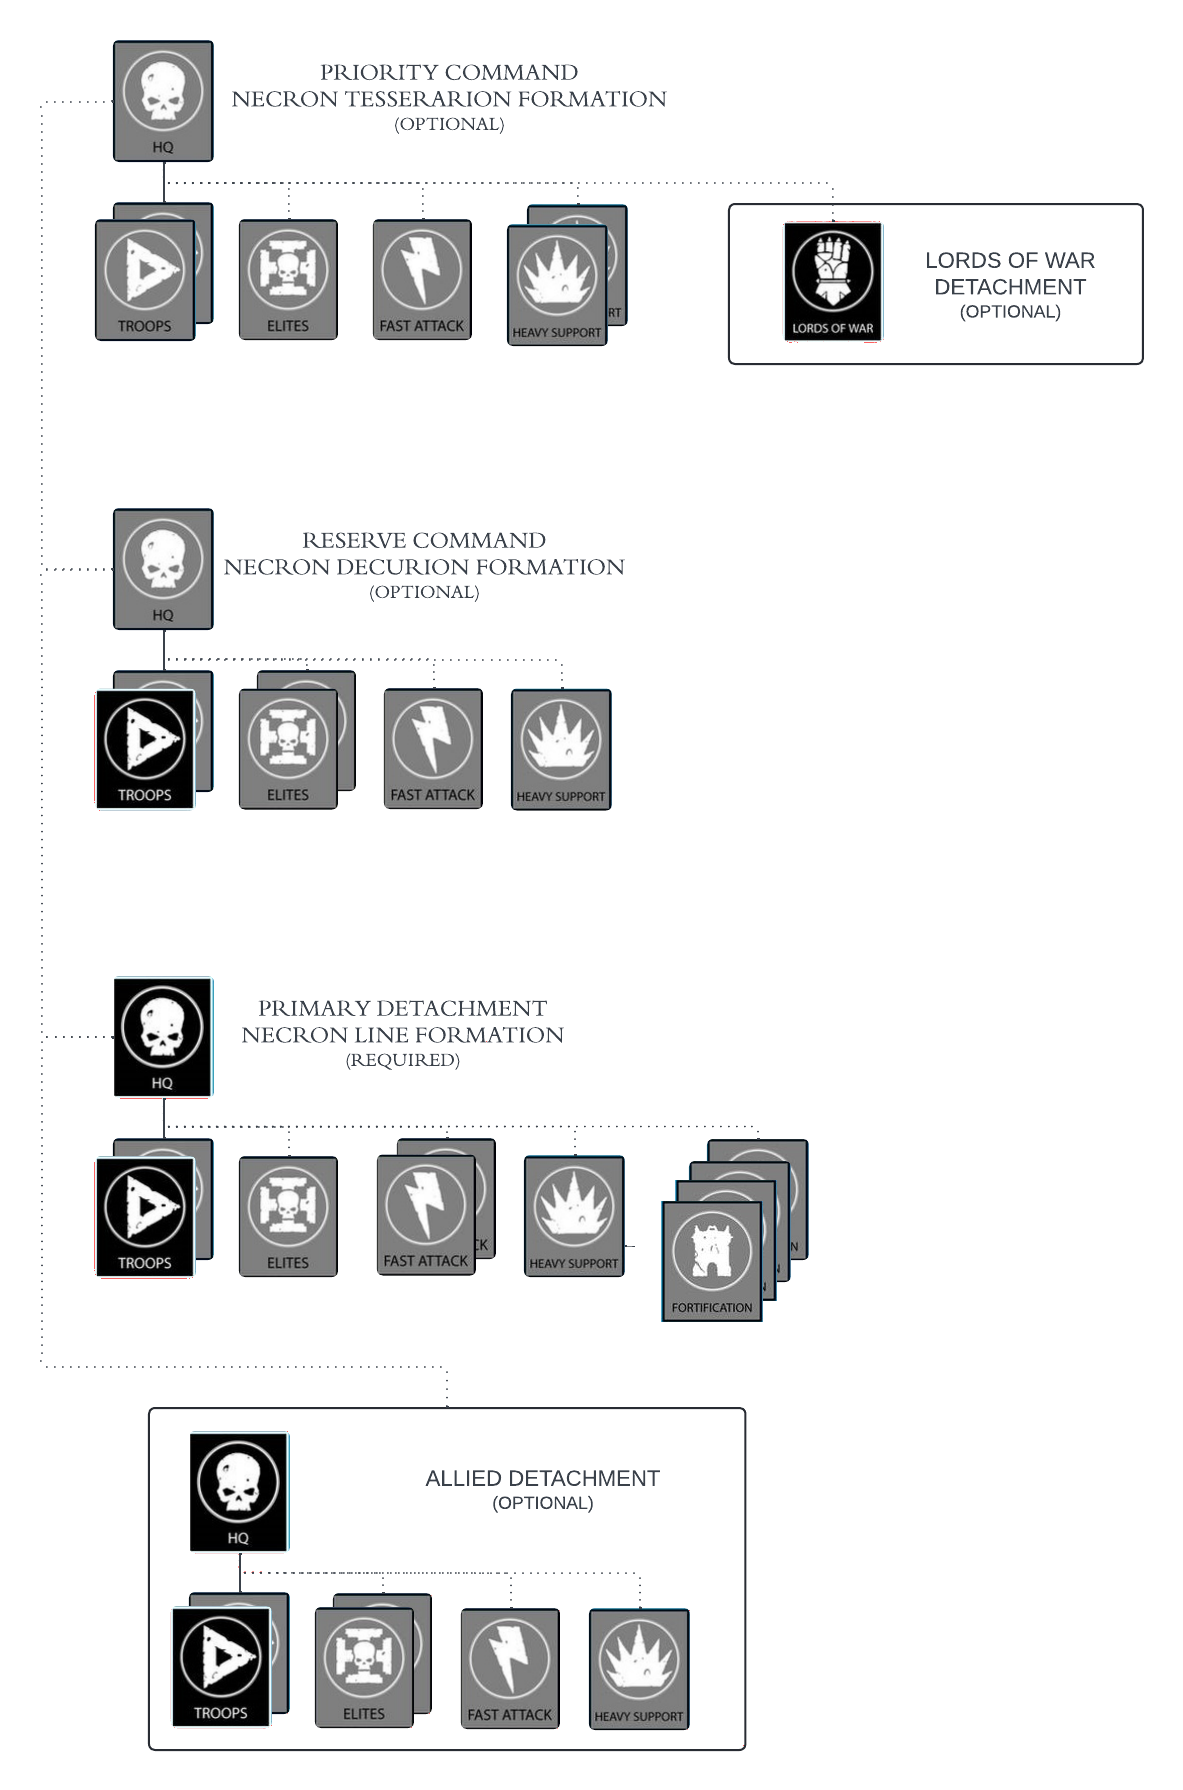
\includegraphics[width=470pt, height=700pt]{Org chart.png}

\begin{figure}
	\centering
	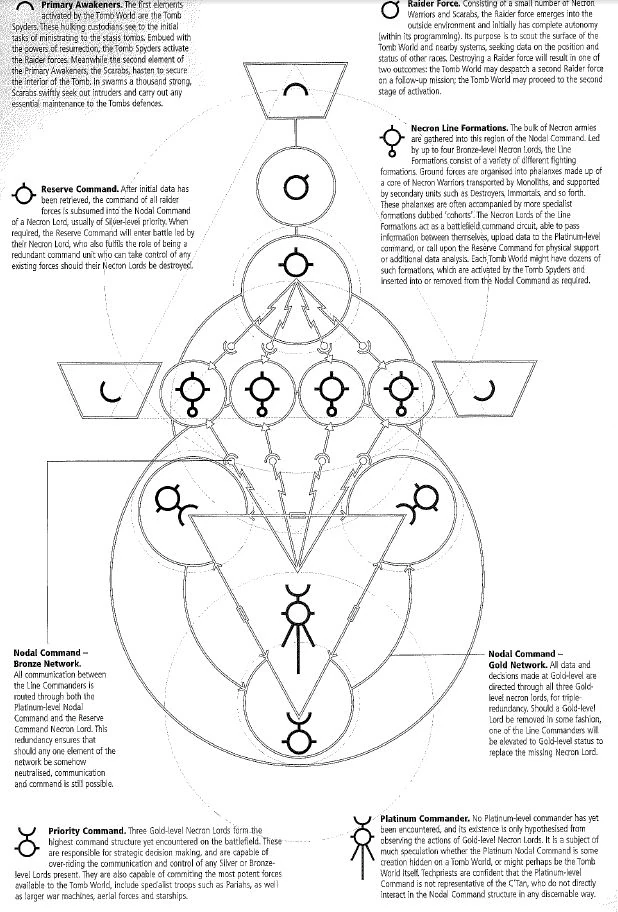
\includegraphics[width=515pt, height=750pt]{nodal.png}
\end{figure}
}

\newpage
\subsection{Warlords of the Necron Dynasties}

\subsubsection{Core Warlord Traits}
These Traits are available to any Character model selected as an army’s Warlord, regardless of Faction or Allegiance.

\begin{multicols}{2}

\textbf{Blood Handed}

\textit{Some warlords are only satisfied by the clash of blades and
the screams of the enemy as they fall before them. For such
warriors, strategy is but a means to an end, a tool by which
they can bring their forces into the brutal crucible of the melee
as soon as possible. There, in the heart of the battlefield, they
seek victory at any cost.}

\vspace*{1em}
Any combat with at least one friendly model within 12"
of this Warlord, or a combat which includes this Warlord,
gains a bonus of +1 to the number of Wounds caused for
the purposes of combat resolution. In addition, an army
whose Warlord has this Trait may make an additional
Reaction during their opponent’s Assault phase as long as
the Warlord has not been removed as a casualty.

\vspace*{1em}
\textbf{Stoic Defender}

\textit{This warlord is a rock, the hard place against which their foes
	are dashed and broken. When the enemy surges forth, they do
	not foolishly go to meet them, but dig in so that the foe may
	exhaust themselves against the defences prepared for them. In
	the end, victory comes to those willing to endure the fires of
	battle and emerge unscathed from its fury.}

\vspace*{1em}
Any friendly unit joined by a Warlord with this Trait
that makes a Shooting Attack will force the target unit to
make a Pinning test if it suffers any unsaved Wounds. In
addition, an army whose Warlord has this Trait may make
an additional Reaction during their opponent’s Shooting
phase as long as the Warlord has not been removed
as a casualty.

\vspace*{1em}
\textbf{Ever-vigilant}

\textit{Always ready to take advantage of the foe’s weakness, this
	warlord is a master of predicting and exploiting the flow of
	battle. Where the foe advances, this warlord falls back to
	better ground, where the foe retreats, this warlord advances,
	for victory is fickle and only falls into the grasp of those
	prepared for any eventuality.}

\vspace*{1em}
When this Warlord, and any unit it has joined, Runs
during the Movement phase, it adds the value of the
Warlord’s Initiative Characteristic, increased by 1, to
the distance moved, rather than the lowest Initiative
Characteristic in the unit. In addition, an army whose
Warlord has this Trait may make an additional Reaction
during their opponent’s Movement phase as long as the
Warlord has not been removed as a casualty.

\end{multicols}

\subsubsection{Necron Warlord Traits}
These Traits are available to any Character model selected as an army’s Warlord, regardless of Faction or Allegiance.

\begin{multicols}{2}
	
	Two or Three Necron Traits + 1 per Dynasty?
	
	\textbf{Sautekh: Hyperlogical Strategist}
	
	One of those ones that gives a reaction in each phase, versatile commander type
	
\end{multicols}
